\documentclass{article}
\title{The survival2 data}
\usepackage{graphicx}
\usepackage{Statweave}
\begin{document}
\maketitle
The data:
\begin{verbatim}
1 1 0 16 
2 1 0 24 
2 1 0 18 
3 0 0 27 
4 1 0 25 
5 1 0 21 
11 1 0 55 
7 1 1 26 
8 1 1 36 
10 1 1 38 
10 0 1 45 
12 1 1 47 
\end{verbatim}
The SAS code and output:
\begin{Winput}
options linesize=70;

data dancers;
  infile "survival1.dat";
  input months dancing treatment age;

proc print;
 
data mypred;
  input treatment age;
  datalines;
  0 25 
  0 45 
  1 25 
  1 45 
;

proc phreg data=dancers;
  model months*dancing(0) = age treatment;
  baseline out=fred covariates=mypred survival=s / nomean;

/*

goptions reset=all;
  
proc gplot;
  plot s*months;

proc gplot;
    plot s*months=age;

*/

data fred2;
  set fred;
  agetrt=cat(age,"-",treatment);  
  
proc print;

goptions reset=all;
symbol1 c=blue v=triangle i=l;
symbol2 c=cyan v=circle i=l;
symbol3 c=red v=diamond i=l;
symbol4 c=black v=plus i=l;

proc gplot;
  plot s*months=agetrt;  

run;

\end{Winput}
\begin{Woutput}
Obs    months    dancing    treatment    age
  1       1         1           0         16
  2       2         1           0         24
  3       2         1           0         18
  4       3         0           0         27
  5       4         1           0         25
  6       5         1           0         21
  7      11         1           0         55
  8       7         1           1         26
  9       8         1           1         36
 10      10         1           1         38
 11      10         0           1         45
 12      12         1           1         47

The PHREG Procedure
          Model Information
Data Set                 WORK.DANCERS
Dependent Variable       months
Censoring Variable       dancing
Censoring Value(s)       0
Ties Handling            BRESLOW

Number of Observations Read          12
Number of Observations Used          12

Summary of the Number of Event and Censored Values
                                     Percent
   Total       Event    Censored    Censored
      12          10           2       16.67

                       Convergence Status
         Convergence criterion (GCONV=1E-8) satisfied.

         Model Fit Statistics
                 Without           With
Criterion     Covariates     Covariates
-2 LOG L          33.573         12.572
AIC               33.573         16.572
SBC               33.573         17.177

        Testing Global Null Hypothesis: BETA=0
Test                 Chi-Square       DF     Pr > ChiSq
Likelihood Ratio        21.0016        2         <.0001
Score                   14.2093        2         0.0008
Wald                     5.5556        2         0.0622

            Analysis of Maximum Likelihood Estimates
              Parameter   Standard                         Hazard
Parameter DF   Estimate      Error Chi-Square Pr > ChiSq    Ratio
age        1   -0.35284    0.14973     5.5532     0.0184    0.703
treatment  1   -4.28283    2.54084     2.8412     0.0919    0.014

Obs    treatment    age    months       s       agetrt
  1        0         25       0      1.00000     25-0
  2        0         25       1      0.97690     25-0
  3        0         25       2      0.87856     25-0
  4        0         25       4      0.72245     25-0
  5        0         25       5      0.56647     25-0
  6        0         25       7      0.00000     25-0
  7        0         25       8      0.00000     25-0
  8        0         25      10      0.00000     25-0
  9        0         25      11      0.00000     25-0
 10        0         25      12      0.00000     25-0
 11        0         45       0      1.00000     45-0
 12        0         45       1      0.99998     45-0
 13        0         45       2      0.99989     45-0
 14        0         45       4      0.99972     45-0
 15        0         45       5      0.99951     45-0
 16        0         45       7      0.91830     45-0
 17        0         45       8      0.14589     45-0
 18        0         45      10      0.00134     45-0
 19        0         45      11      0.00000     45-0
 20        0         45      12      0.00000     45-0
 21        1         25       0      1.00000     25-1
 22        1         25       1      0.99968     25-1
 23        1         25       2      0.99821     25-1
 24        1         25       4      0.99552     25-1
 25        1         25       5      0.99219     25-1
 26        1         25       7      0.25528     25-1
 27        1         25       8      0.00000     25-1
 28        1         25      10      0.00000     25-1
 29        1         25      11      0.00000     25-1
 30        1         25      12      0.00000     25-1
 31        1         45       0      1.00000     45-1
 32        1         45       1      1.00000     45-1
 33        1         45       2      1.00000     45-1
 34        1         45       4      1.00000     45-1
 35        1         45       5      0.99999     45-1
 36        1         45       7      0.99882     45-1
 37        1         45       8      0.97378     45-1
 38        1         45      10      0.91271     45-1
 39        1         45      11      0.62315     45-1
 40        1         45      12      0.08223     45-1
\end{Woutput}
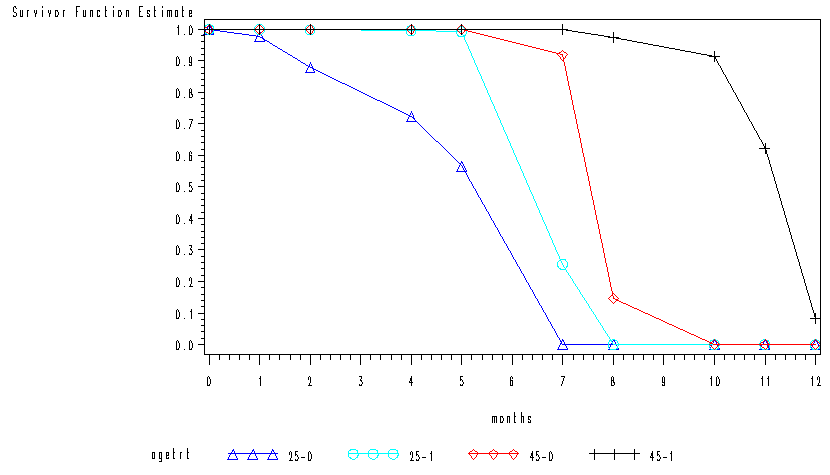
\includegraphics[width=4in]{survival-curves}
\end{document}
